\documentclass[]{article}
\usepackage[T1]{fontenc}
\usepackage{graphicx}
\usepackage{tabularborder}
\usepackage{booktabs}
\usepackage{tabularx}
\usepackage{float}
\usepackage{tikz}
\usepackage{placeins}
\usepackage{scrextend}
\usepackage{caption}
\usetikzlibrary{shapes}
\usetikzlibrary{fit}
\usepackage{fancyhdr}
\pagestyle{fancy}
\fancyhf{}
\renewcommand{\headrulewidth}{0pt}
\renewcommand{\footrulewidth}{0pt}
\fancyfoot[C]{\thepage}
\usepackage{graphicx}
\usepackage{amsmath}
\usepackage{pgfplots}
\usepackage{float}
\usepackage[margin=1.2in]{geometry}
\usepackage[spanish]{babel}
\usepackage{amsmath}
\usepackage{amssymb}
\usepackage{caption}
\usepackage{subcaption}
\usepackage{graphicx}
\newcommand{\dint}{\delta_{\text{int}}}
\newcommand{\dext}{\delta_{\text{ext}}}
\newcommand{\estado}{(cid,ls,\sigma)}
\newcommand{\mediatorstate}{(b,r,c,sr,br\sigma)}
\newcommand{\R}{\mathbb{R}}
\newcommand{\N}{\mathbb{N}}
\pgfplotsset{compat=1.16}
\title{\textbf{Implementación del Juego de la vida de Conway's en PowerDEVS}}
\author{Lucio Mansilla - Brenda Dichiara}
\date{\today}
\begin{document}
\maketitle

\section{Introducción / Problema}
El Juego de la Vida de Conway's, comúnmente conocido como "Juego de la Vida", es un autómata celular que fue propuesto por el matemático británico John Horton Conway en 1970. Los autómatas celulares son modelos matemáticos para sistemas dinámicos que evolucionan en pasos de tiempo discretos(generaciones). A pesar de su simplicidad aparente, tienen la capacidad de simular sistemas complejos y mostrar comportamientos emergentes, siendo utilizados en diversos contextos, desde la física hasta la teoría de computación.

En el Juego de la Vida, cada celda que compone la cuadricula bidimensional puede estar en uno de dos estados: $viva$ o $muerta$. Las celdas interactúan con sus ocho vecinos adyacentes en horizontal, vertical y diagonal, transicionando entre los estados de vida y muerte de acuerdo a las siguientes reglas de evolución en su versión original:

\begin{itemize}
  \item Cualquier celda viva con dos o tres vecinos vivos sobrevive para la siguiente generación.
  \item Cualquier celda viva con menos de dos vecinos vivos muere por soledad/aislamiento para la siguiente generación.
  \item Cualquier celda viva con más de tres vecinos vivos muere por sobrepoblación para la siguiente generación.
  \item Cualquier celda muerta con exactamente tres vecinos vivos nace para la siguiente generación.
\end{itemize}

Estas reglas originales son comúnmente denotadas como 23/3, representando las condiciones de supervivencia y nacimiento, respectivamente. Es decir, una celda viva sobrevive si tiene 2 o 3 vecinos vivos y una celda muerta nace si tiene exactamente 3 vecinos vivos.

Se han desarrollado una gran cantidad de variantes. En este sistema de reglas, la denominación "S/B" (Survive/Birth) representa las condiciones para la supervivencia y el nacimiento de las células. "S" son los números de vecinos que permiten a una celda viva sobrevivir, y "B" son los números de vecinos que permiten a una celda muerta nacer. Algunas variantes que podemos destacar:

\begin{itemize}
  \item HighLife: 23/36. Similar al Juego de la Vida original, pero con la adición de que las células muertas con 6 vecinos vivos también nacen. Este juego es famoso por su patrón "replicator", el primero que se descubrió y que puede replicarse a sí mismo.
  \item Seeds: 0/2. En esta variante, las células vivas no sobreviven y las células muertas nacen si tienen exactamente 2 vecinos vivos. Es conocido por su crecimiento muy rápido y la creación de estructuras complejas a partir de pequeñas semillas.
\end{itemize}

Es importante señalar que la mayoría de las $2^18$ posibles reglas del espacio producen universos que son o bien demasiado caóticos, o bien demasiado desolados para ser de interés. Sin embargo, es posible observar la aparición de diversos patrones, algunos  estáticos, otros oscilan entre varios estados y otros se desplazan por el tablero. Estos patrones serán el objeto de estudio en las secciones posteriores de este informe.

El propósito de este proyecto es explorar la dinámica del juego de una manera visual e interactiva. Para ello, se implementará el juego en PowerDEVS, una herramienta de simulación de eventos discretos basada en la teoría DEVS (Discrete Event System Specification).

\section{Especificación DEVS de una celda}\label{sec:esp}


El DEVS que representa únicamente a una célula se define como sigue:

\[ C = \langle X, Y, S, \dint, \dext, \lambda, ta \rangle \]

donde

\begin{itemize}
  \item $X = GameState$


        La estructura de $GameState$ se define formalmente como sigue:

        \begin{itemize}
          \item \textbf{board}: Un conjunto que representa el estado de cada célula en el tablero del juego. Cada celda en el tablero puede tener un valor de 0 (muerta) o 1 (viva).
          \item \textbf{rows}: El número total de filas en el tablero.
          \item \textbf{cols}: El número total de columnas en el tablero.
          \item \textbf{SR}: Representa las reglas de supervivencia.
          \item \textbf{BR}: Representa las reglas de nacimiento.
        \end{itemize}



  \item $Y = \N \times \{0,1\}$

  \item $S = \N \times \{0, 1\} \times  \R_0^+$

        El estado es una tupla $(cid, ls, \sigma)$ donde

        \begin{itemize}
          \item $cid \in \N$ es el identificador de la célula.
          \item $ls \in \{0, 1\}$ es el estado de la célula (1 = viva, 0 = muerta)
          \item $\sigma \in \R_0^+$ es el tiempo restante para realizar una próxima salida.
        \end{itemize}

  \item $\dint(\estado) = (cid,ls,\infty)$

  \item $\dext(\estado, e, (x, p)) = \begin{cases}
            (cid,0,1)  & ls = 1 \ \land \ alives \ \not \in x.SR \\
            (cid,1,1)  & ls = 0 \ \land \ alives \in x.BR        \\
            (cid,ls,1) & \text{otherwise }
          \end{cases}$

        donde $alives = \text{countAlives}(x.rows,x.cols,cid,x.board)$
  \item $\lambda(\estado) = (cid,ls) $
  \item $ta(\estado) = \sigma$
\end{itemize}

Donde $x.SR$ y $x.BR$ representan las reglas de supervivencia y nacimiento respectivamente, las cuales se explican en detalle en la Sección 1: $"$Introducción / Problema$"$.

\begin{itemize}
  \item \textbf{countAlives}: Esta función es responsable de determinar la cantidad de células vecinas vivas para una célula específica. Se le proporcionan cuatro parámetros claves: el número de filas (rows) y columnas (cols) del tablero, el identificador único de la célula (cell\_id) y el estado actual del tablero (board). La función realiza tres pasos principales:

        \begin{addmargin}[1em]{0em}
          \begin{itemize}
            \item \textbf{Identificación}: Localiza la posición exacta de la célula dada en el tablero utilizando su identificador y las dimensiones del tablero.
            \item \textbf{Exploración y Conteo}: Examina únicamente las células vecinas, excluyendose a sí misma, y realiza un conteo de cuantas vecinas estan vivas.
            \item \textbf{Resultado}: Retorna la cantidad total de células vecinas vivas.
          \end{itemize}
        \end{addmargin}
\end{itemize}

\subsection{Mediator}
\paragraph{}
Como podemos apreciar, la lógica de cada célula en DEVS es relativamente sencilla. Esto se debe, en gran medida, a la presencia de un patrón de diseño muy popular en la programación, conocido como \textit{Mediator}. El Mediator permite desacoplar la lógica de las células, gestionar el tiempo de los eventos y distribuir la información del tablero. Es un patrón de diseño de comportamiento que se utiliza para reducir las comunicaciones complejas y las dependencias entre diferentes entidades.\\

En el contexto de DEVS, el \textit{Mediator} se encarga de transmitir el estado inicial, así como cualquier cambio en el tablero a las células individuales. A su vez, las células informan al \textit{Mediator} sobre cualquier cambio de estado. Este proceso permite que la información se distribuya de manera independiente entre todas las células.\\

Esta estrategia trae consigo una serie de ventajas significativas. En primer lugar, se simplifica el diseño de las células al no tener que lidiar con la lógica adicional para manejar los tiempos sincronizados de los eventos discretos (Por ejemplo, tener que primero actualizar y luego informar o viceversa). En segundo lugar, al eliminar la necesidad de que cada célula esté directamente conectada con todas las demás, se obtiene un sistema más flexible independiente y escalable, puesto que en un futuro solo basta con añadir una nueva célula y conectarla al \textit{Mediator} para que esta pueda interactuar con el resto del sistema siempre que se obtenga un tablero de $n$ filas y $m$ columnas.\\

La especificación DEVS del \textit{Mediator} se puede describir como:

\[ M = \langle X, Y, S, \dint, \dext, \lambda, ta \rangle \]


\begin{itemize}
  \item $X = \N \times \{0,1\}$

  \item $Y = GameState$

  \item $S = GameState \times  \R_0^+$\\

        definiendo game $\in$ $GameState$ entonces se tiene:
  \item $\dint(game,\sigma) = (game,\infty)$

  \item $\dext(game, \sigma, (cell\_id, life\_state)) =
          (game.board[x.cell\_id] \leftarrow x.life\_state, 1)
        $


  \item $\lambda(game) = game $
  \item $ta(game,\sigma) = \sigma$
\end{itemize}


\subsection{Primer optimización}

\subsection{Segunda optimización}
% Aquí iría la especificación formal del Mediator.






% Aquí puedes detallar cómo especificaste una celda del juego en DEV
\section{Implementación en PowerDEVS}
% En esta sección puedes describir los patrones que has implementado.
En PowerDEVS, el juego de la vida se implementa utilizando dos componentes clave: una entidad denominada 'célula' y un patrón de diseño denominado 'mediator'. Ambos son modelos atómicos y sus relaciones e interacciones definen el estado y el comportamiento del juego.

La célula se implementa como un modelo atómico simple con una única entrada y salida. Cada célula es una entidad única que cuenta con un identificador único que la representa en el tablero. Por otro lado, el Mediator es un modelo que juega un papel crucial para coordinar y gestionar las interacciones entre estas células.

El Mediator, también implementado como un modelo atómico, desempeña un papel central en la coordinación y el control de las interacciones entre las células. Este componente no solo gestiona las relaciones entre las células, sino que también es responsable de inicializarlas. El Mediator recibe como parámetro el nombre del archivo que contiene el estado inicial del tablero asi como las reglas de supervivencia y nacimiento (1er parámetro). Además una de las funcionalidades importantes del Mediator es que permite definir el nombre de archivo de salida (2do parámetro), en el mismo se registra el estado del tablero del juego en cada generación, facilitando su exportación y visualización en formatos como gif, mp4 o png.

En la Figura \ref{fig:cell_mediator} a la izquierda se muestra la representación de una célula como un modelo atómico, y a la derecha, el Mediator.

\begin{figure}[H]
  \centering
  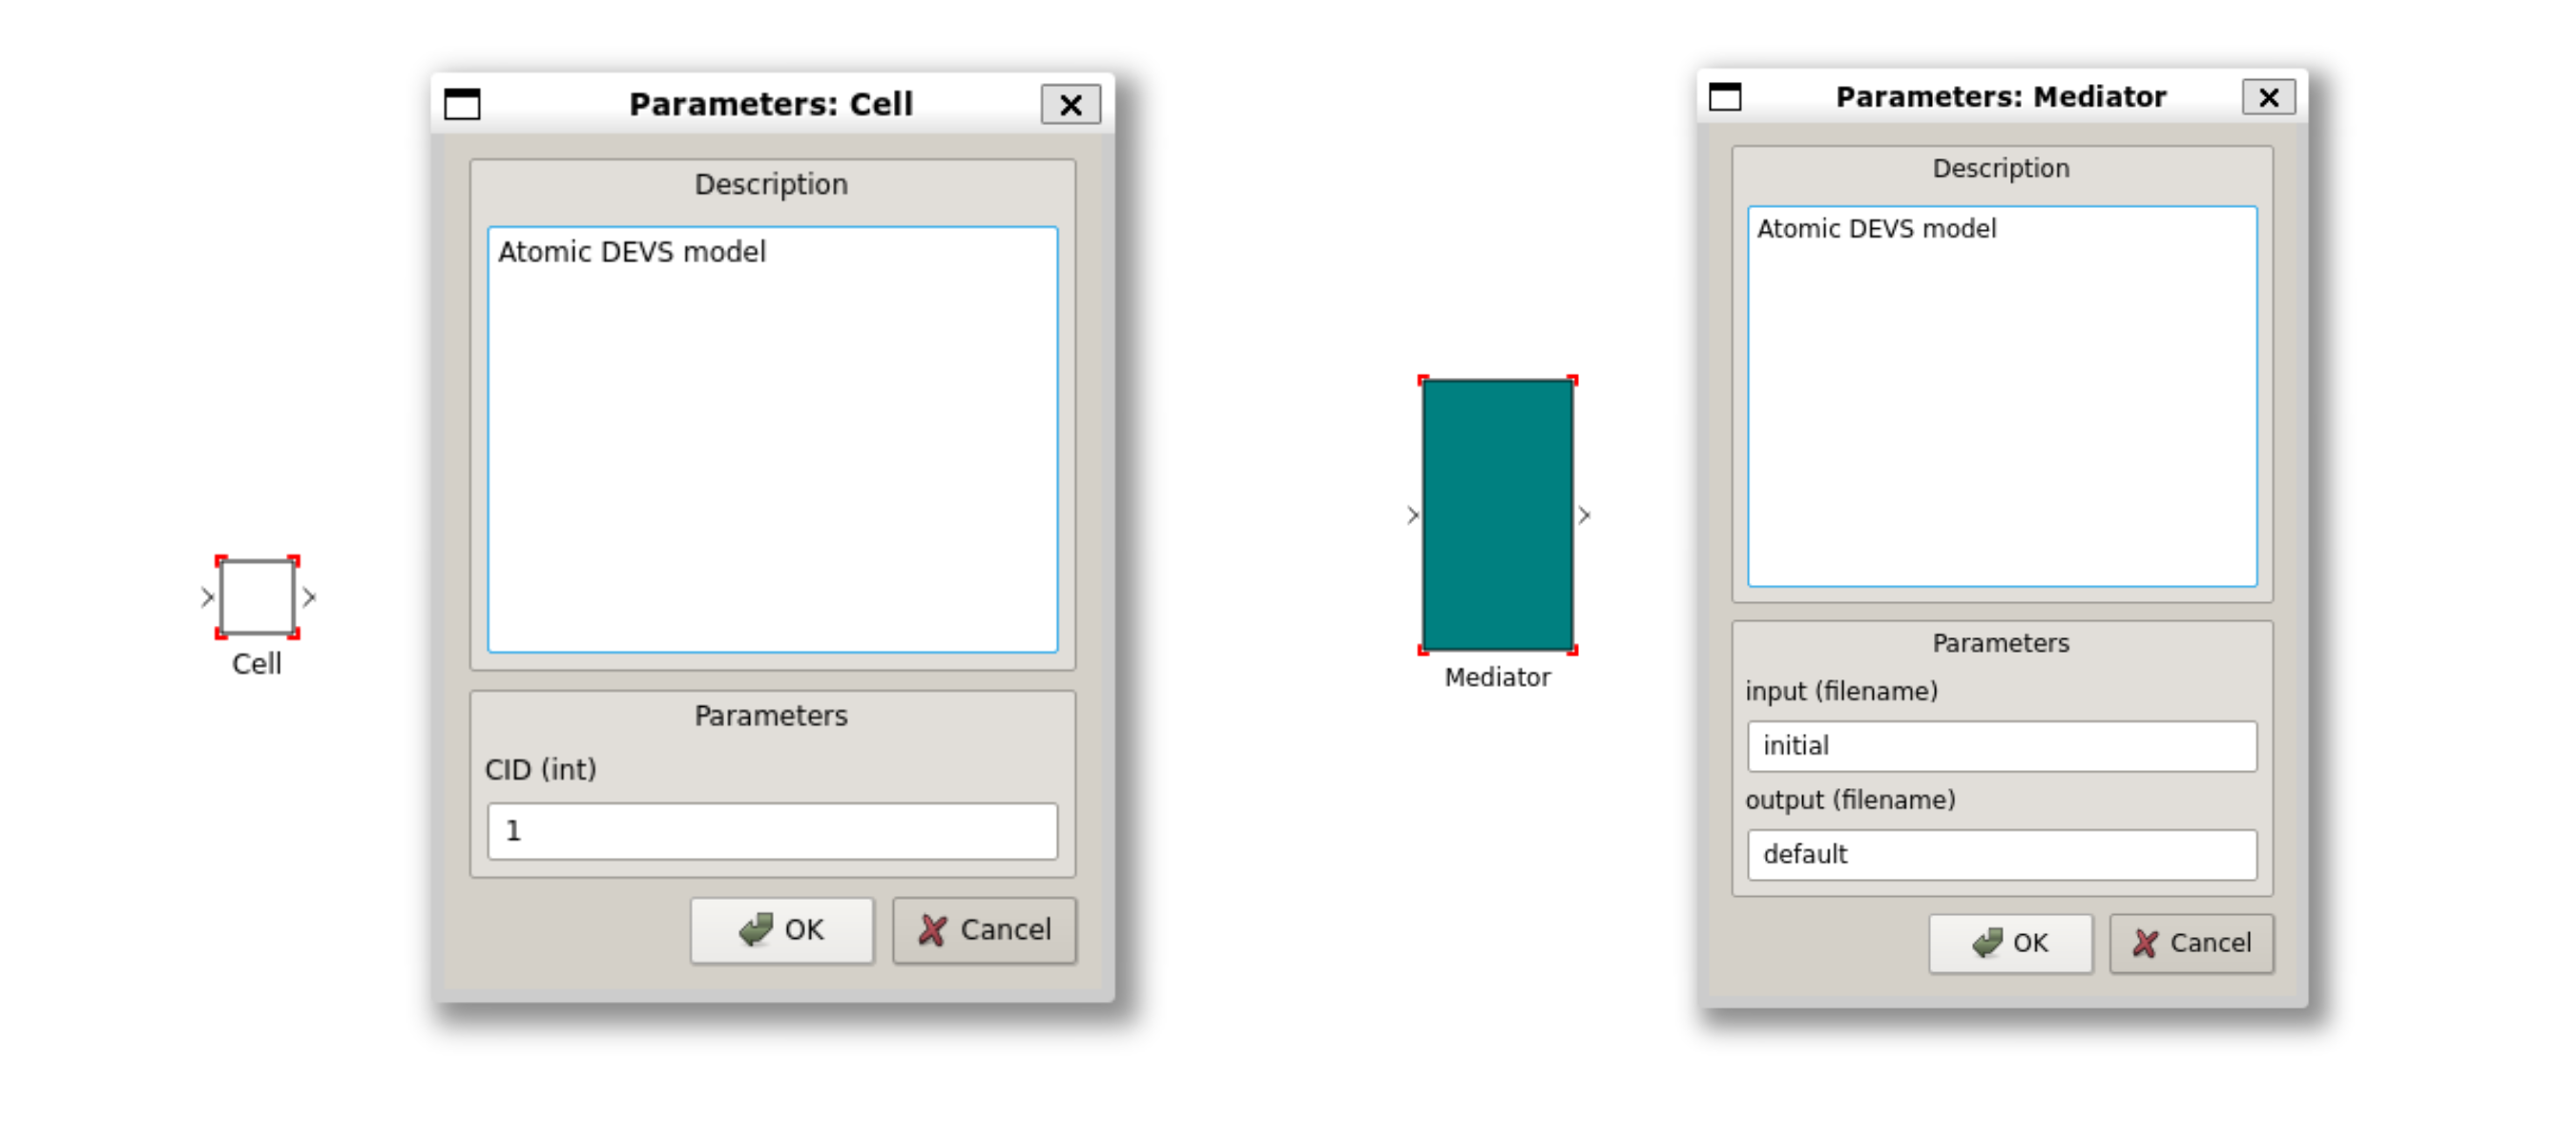
\includegraphics[width=1\textwidth]{../assets/pdevs/mediator_cell.png}
  \caption{El Mediator y la Célula como modelos atómicos en PowerDEVS.}
  \label{fig:cell_mediator}
\end{figure}

El trabajo conjunto de estas dos entidades da lugar a la dinámica del juego. A través del Mediator, el juego inicializa y coordina el estado de las células, gestionando su comportamiento a lo largo de cada generación. En la siguiente imagen, se proporcionará un ejemplo de un tablero de 3x3 inicializado por un Mediator, ilustrando cómo se interconectan múltiples células y cómo el Mediator permite que cada célula sea independiente de las demás, es decir, no se comunican directamente entre ellas.

\begin{figure}[H]
  \centering
  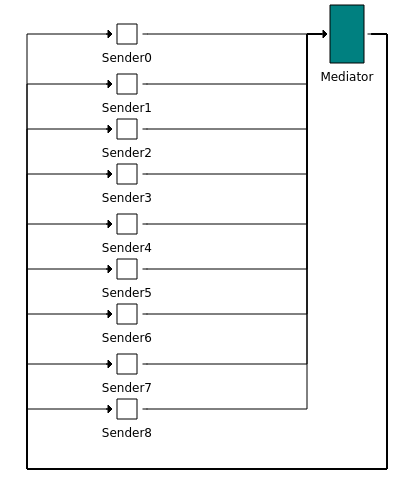
\includegraphics[width=0.4\textwidth]{../assets/pdevs/3x3_board.png}
  \caption{Tablero de ejemplo 3x3.}
  \label{fig:board}
\end{figure}

También se incorporó al proyecto una librería, en la misma se pueden encontrar los modelos atómicos anteriormente mencionados en las \ref{fig:cell_mediator} y \ref{fig:board}, así como también varios modelos de tableros de ejemplo, como se puede observar en la figura \ref{fig:library}.

\begin{figure}[H]
  \centering
  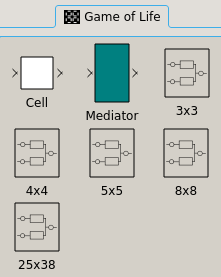
\includegraphics[width=0.3\textwidth]{../assets/pdevs/library.png}
  \caption{Librería}
  \label{fig:library}
\end{figure}

\subsection{Automatización y Personalización de Tableros}

Entendemos que la creación de tableros personalizados en PowerDEVS puede ser un proceso laborioso, especialmente para tableros de grandes dimensiones. Para facilitar este proceso, hemos desarrollado una herramienta de ayuda basada en una interfaz gráfica de usuario (GUI) implementada en Python.

Esta herramienta, que hemos llamado 'Settings GoL', permite generar tableros de dimensiones NxM en formato PDM, los cuales pueden ser utilizados directamente en PowerDEVS. El proceso es sencillo e intuitivo, y reduce significativamente el tiempo y el esfuerzo requeridos para la configuración de tableros personalizados.

En la Figura \ref{fig:settingsdevs}, se muestra una vista previa de la interfaz de Settings GoL y de algunas de sus funcionalidades.

\begin{figure}[H]
  \centering
  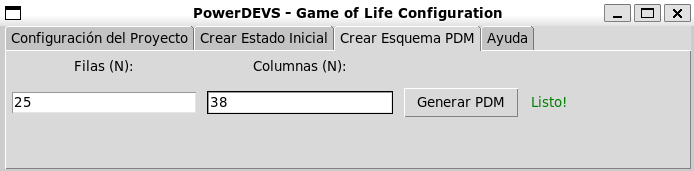
\includegraphics[width=1\textwidth]{../assets/pdevs/SettingsDevs.png}
  \caption{Vista previa de Settings GoL, pestaña generador de tableros PDM.}
  \label{fig:settingsdevs}
\end{figure}

Para un entendimiento completo de cómo utilizar esta herramienta y sus otras funcionalidades se ha elaborado una guía detallada de uso que se encuentra en el anexo de este informe.


\section{Patrones}
El Juego de la Vida, concebido por el matemático británico John Horton Conway, es famoso por la vasta variedad de patrones que emergen de sus simples reglas, en particular, las reglas 23/3. Los patrones se definen como configuraciones de células que se repiten tras un número determinado de generaciones, también conocido como su "periodo". Los patrones pueden ser estáticos, oscilantes o móviles, dependiendo de cómo cambian a lo largo del tiempo. En las secciones siguientes se presentarán ejemplos de estos patrones bajo las reglas 23/3.

\subsection{Patrones estáticos}
Los patrones estáticos, también conocidos como "still lifes", son configuraciones de células que no cambian de una generación a la siguiente, es decir, su periodo es 1. A continuación, se presentan ejemplos de estos patrones:

\begin{figure}[H]
  \centering
  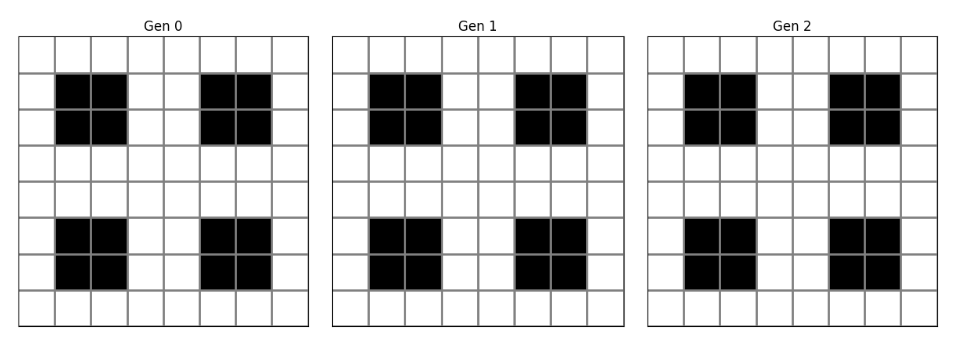
\includegraphics[width=0.75\textwidth]{../assets/still_life/block/block.png}
  \caption{Patrón bloque: un patrón estático compuesto por un cuadrado de 2x2 células. Aparece frecuentemente debido a su simplicidad.}
  \label{fig:block}
\end{figure}

\begin{figure}[H]
  \centering
  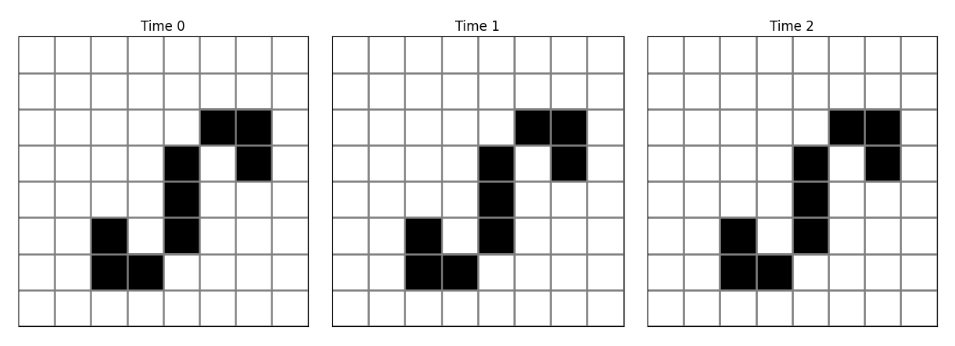
\includegraphics[width=0.75\textwidth]{../assets/still_life/integral/integral.png}
  \caption{Patrón integral: este patrón estático se asemeja a la forma de un signo integral.}
  \label{fig:integral}
\end{figure}

\begin{figure}[H]
  \centering
  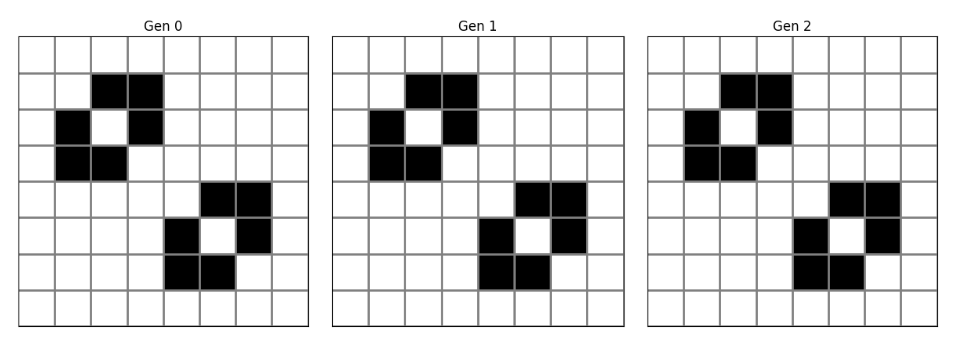
\includegraphics[width=0.75\textwidth]{../assets/still_life/ship/ship.png}
  \caption{Patrón ship: este patrón estático se asemeja a la forma de una nave espacial.}
  \label{fig:ship}
\end{figure}

\begin{figure}[H]
  \centering
  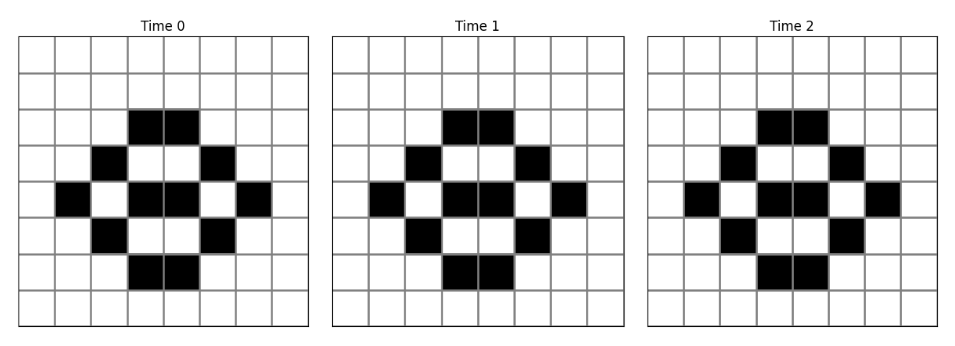
\includegraphics[width=0.75\textwidth]{../assets/still_life/honeycomb/honeycomb.png}
  \caption{Patrón honeycomb: este patrón estático se asemeja a la estructura de un panal de abejas.}
  \label{fig:honeycomb}
\end{figure}

\subsection{Osciladores}
Los osciladores son patrones que vuelven a su configuración inicial después de un número fijo de generaciones, conocido como su período. A diferencia de los patrones estáticos, los osciladores cambian su apariencia durante su ciclo de vida, pero eventualmente vuelven a su estado original.

\begin{figure}[H]
  \centering
  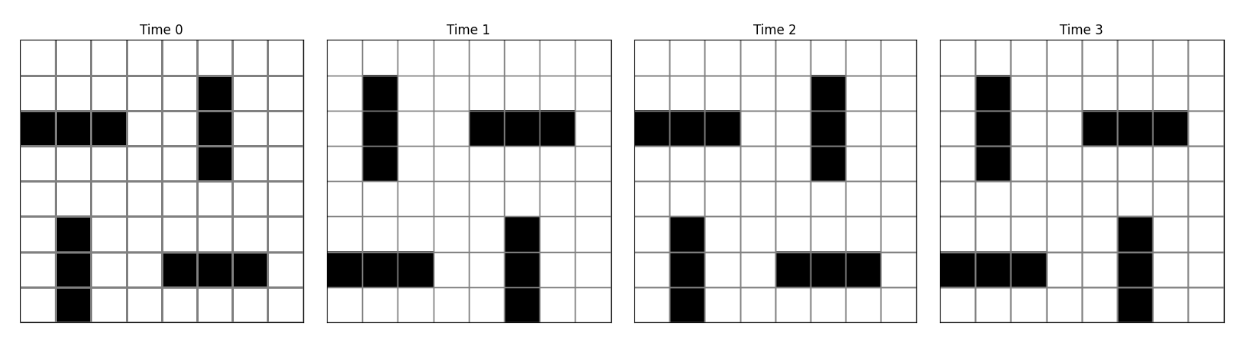
\includegraphics[width=0.9\textwidth]{../assets/oscillator/blinker/blinker.png}
  \caption{Patrón blinker: un oscilador de periodo 2. Oscila entre una orientación horizontal y vertical cada generación. Notar que en este caso hay 4 blinkers en el tablero.}
  \label{fig:blinker}
\end{figure}

\begin{figure}[H]
  \centering
  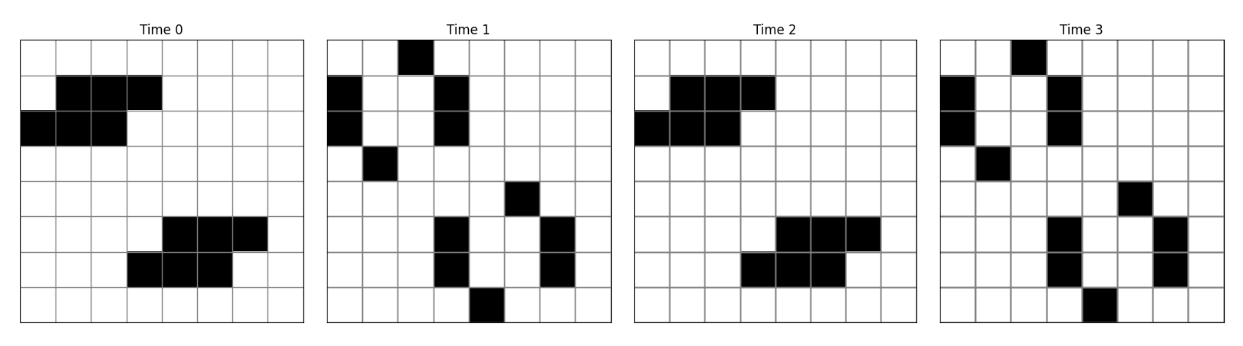
\includegraphics[width=0.9\textwidth]{../assets/oscillator/toad/toad.png}
  \caption{Patrón toad: un oscilador de periodo 2 que oscila entre dos configuraciones.}
  \label{fig:toad}
\end{figure}

\begin{figure}[H]
  \centering
  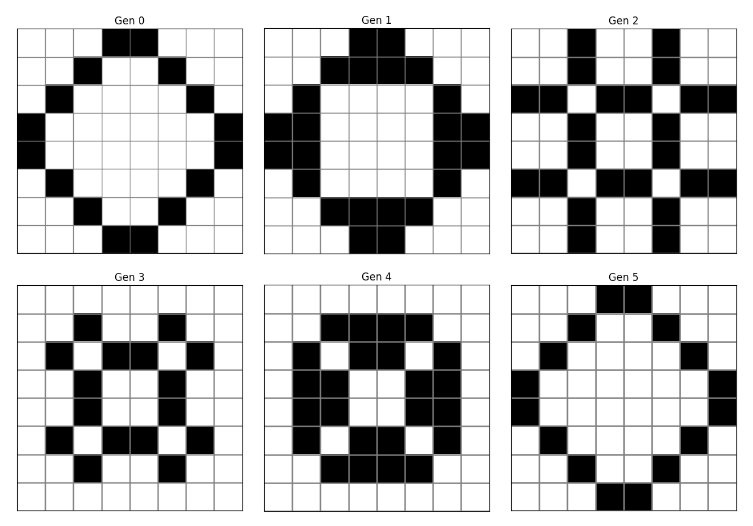
\includegraphics[width=0.7\textwidth]{../assets/oscillator/octagon_2/octagon_2.png}
  \caption{Patrón octagon: un oscilador de periodo 5 que se desplaza en un ciclo de rotación.}
  \label{fig:octagon}
\end{figure}

\begin{figure}[H]
  \centering
  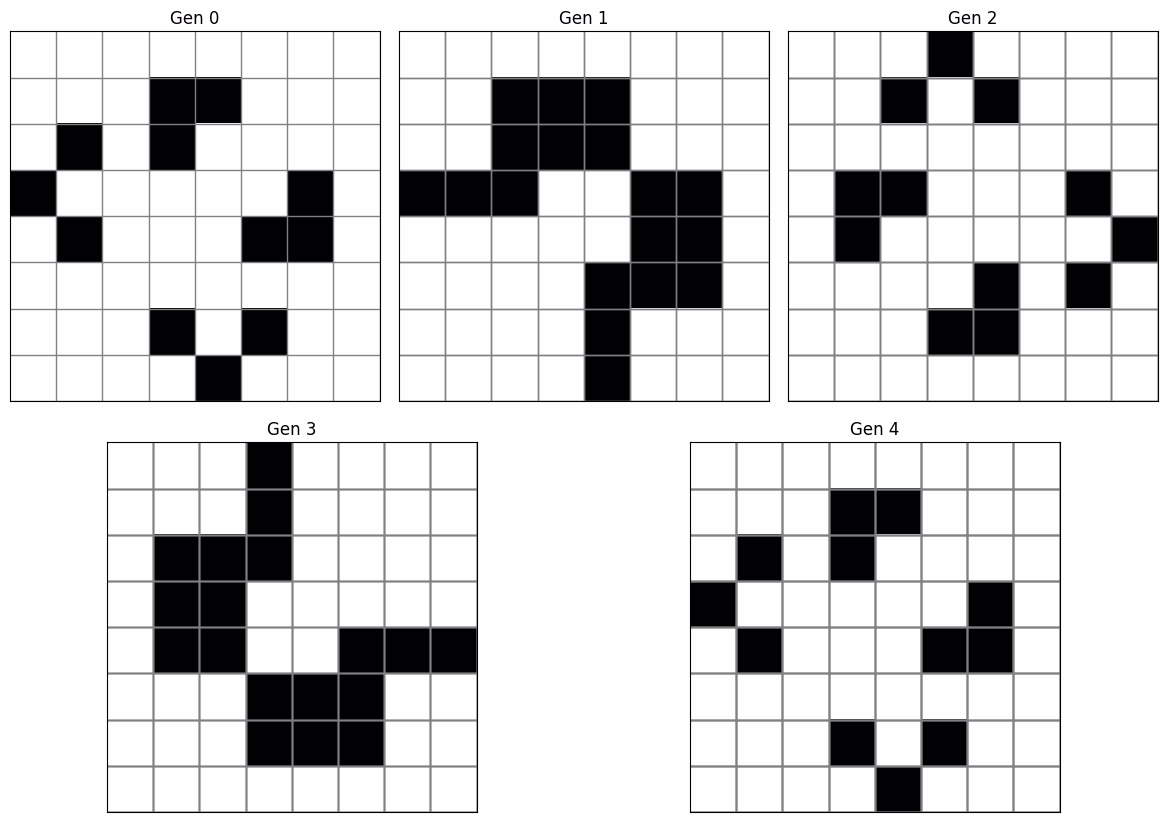
\includegraphics[width=0.7\textwidth]{../assets/oscillator/mazing/mazing.jpg}
  \caption{Patrón mazing: un oscilador de periodo 4 que oscila entre una forma cuadrada y una forma de cruz.}
  \label{fig:mazing}
\end{figure}

\subsection{Naves espaciales}
Las naves espaciales son patrones que se trasladan a través de la cuadrícula mientras oscilan. El ejemplo más conocido es la "nave ligera" (o "glider" en inglés), que se desplaza diagonalmente a través de la cuadrícula mientras oscila entre cuatro configuraciones diferentes.
\begin{figure}[H]
  \centering
  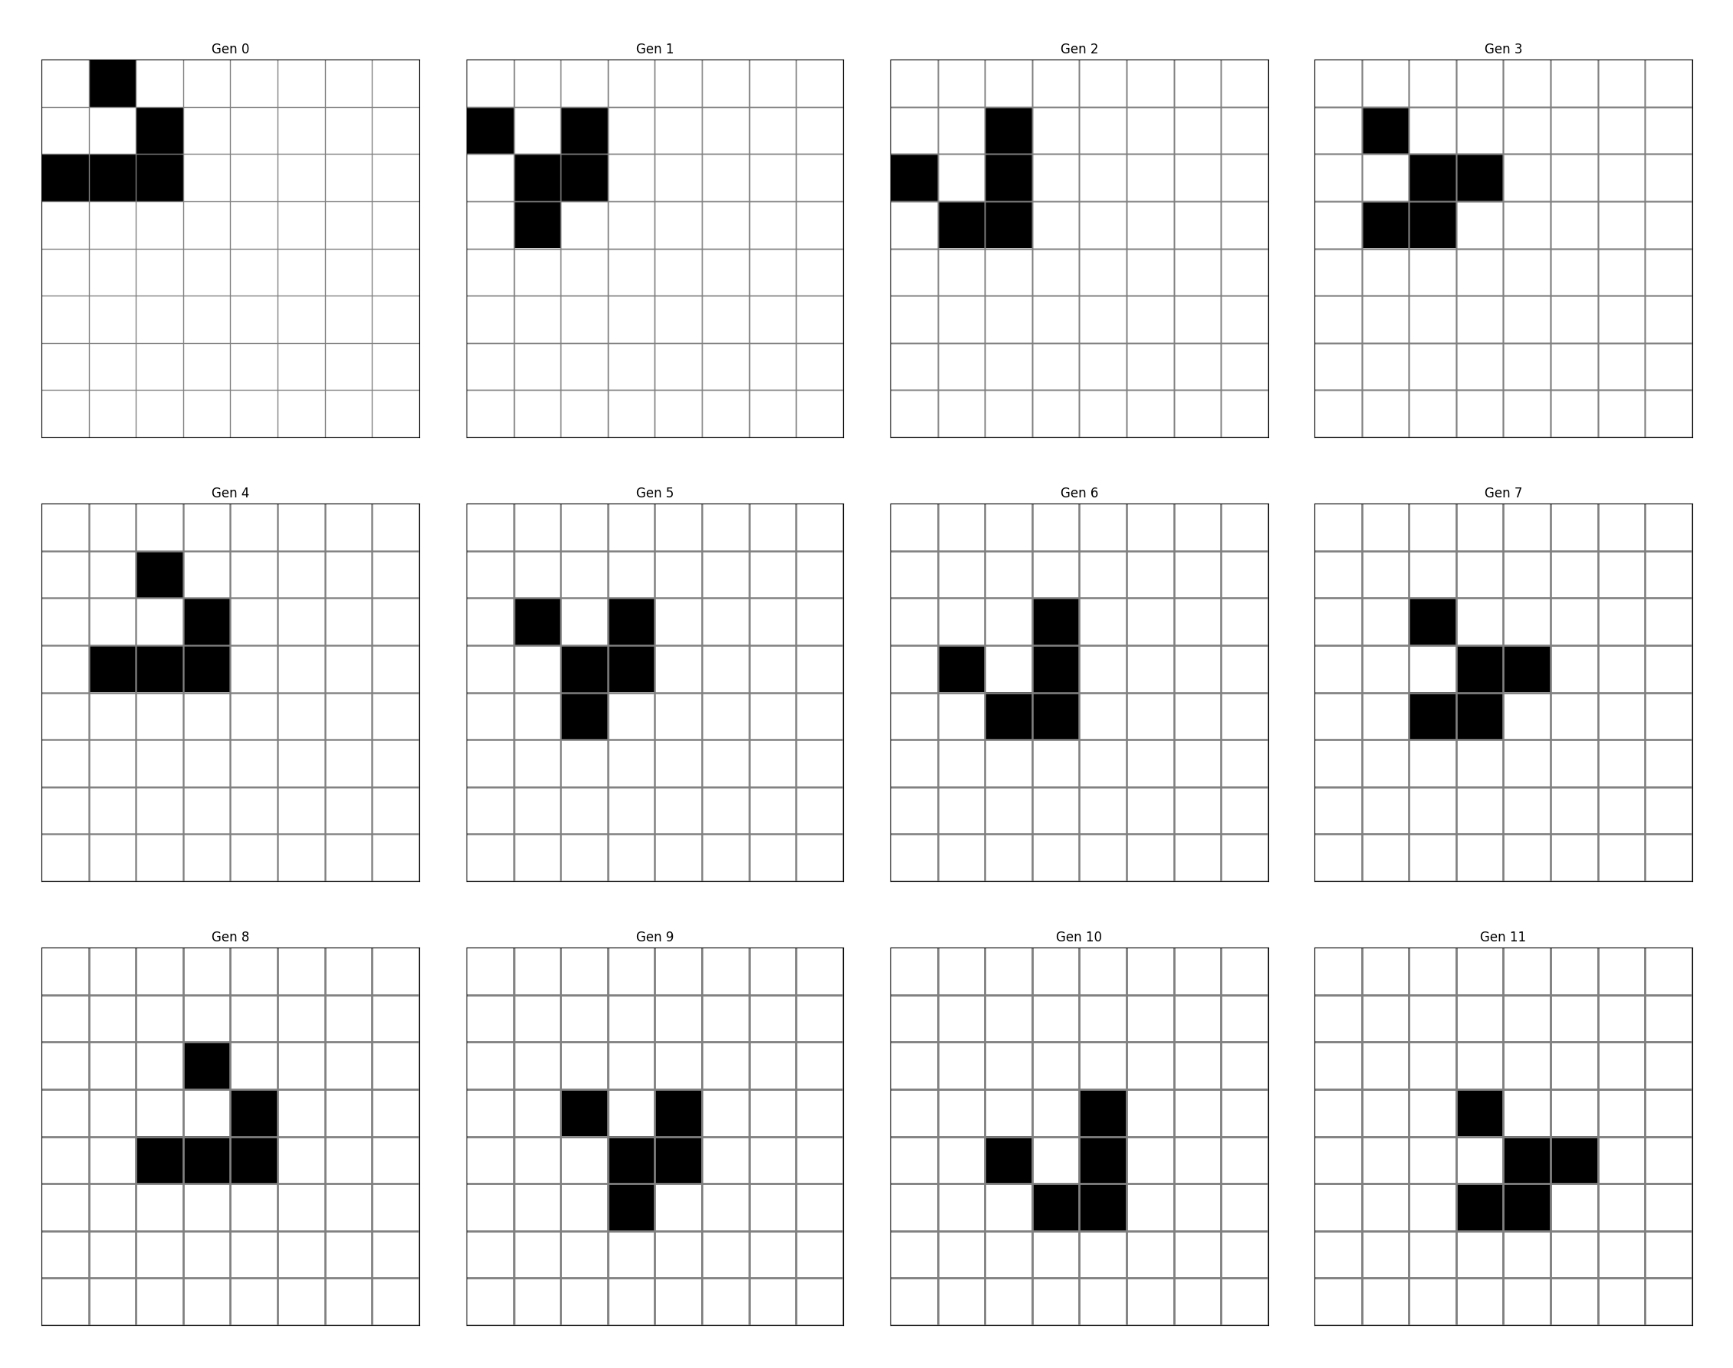
\includegraphics[width=0.87\textwidth]{../assets/space_ships/glider/glider_12.jpg}

  \label{fig:glider}
\end{figure}
\vspace*{-10mm} % Reduce el espacio vertical aquí. Ajusta el valor según sea necesario.
\begin{figure}[H]
  \centering
  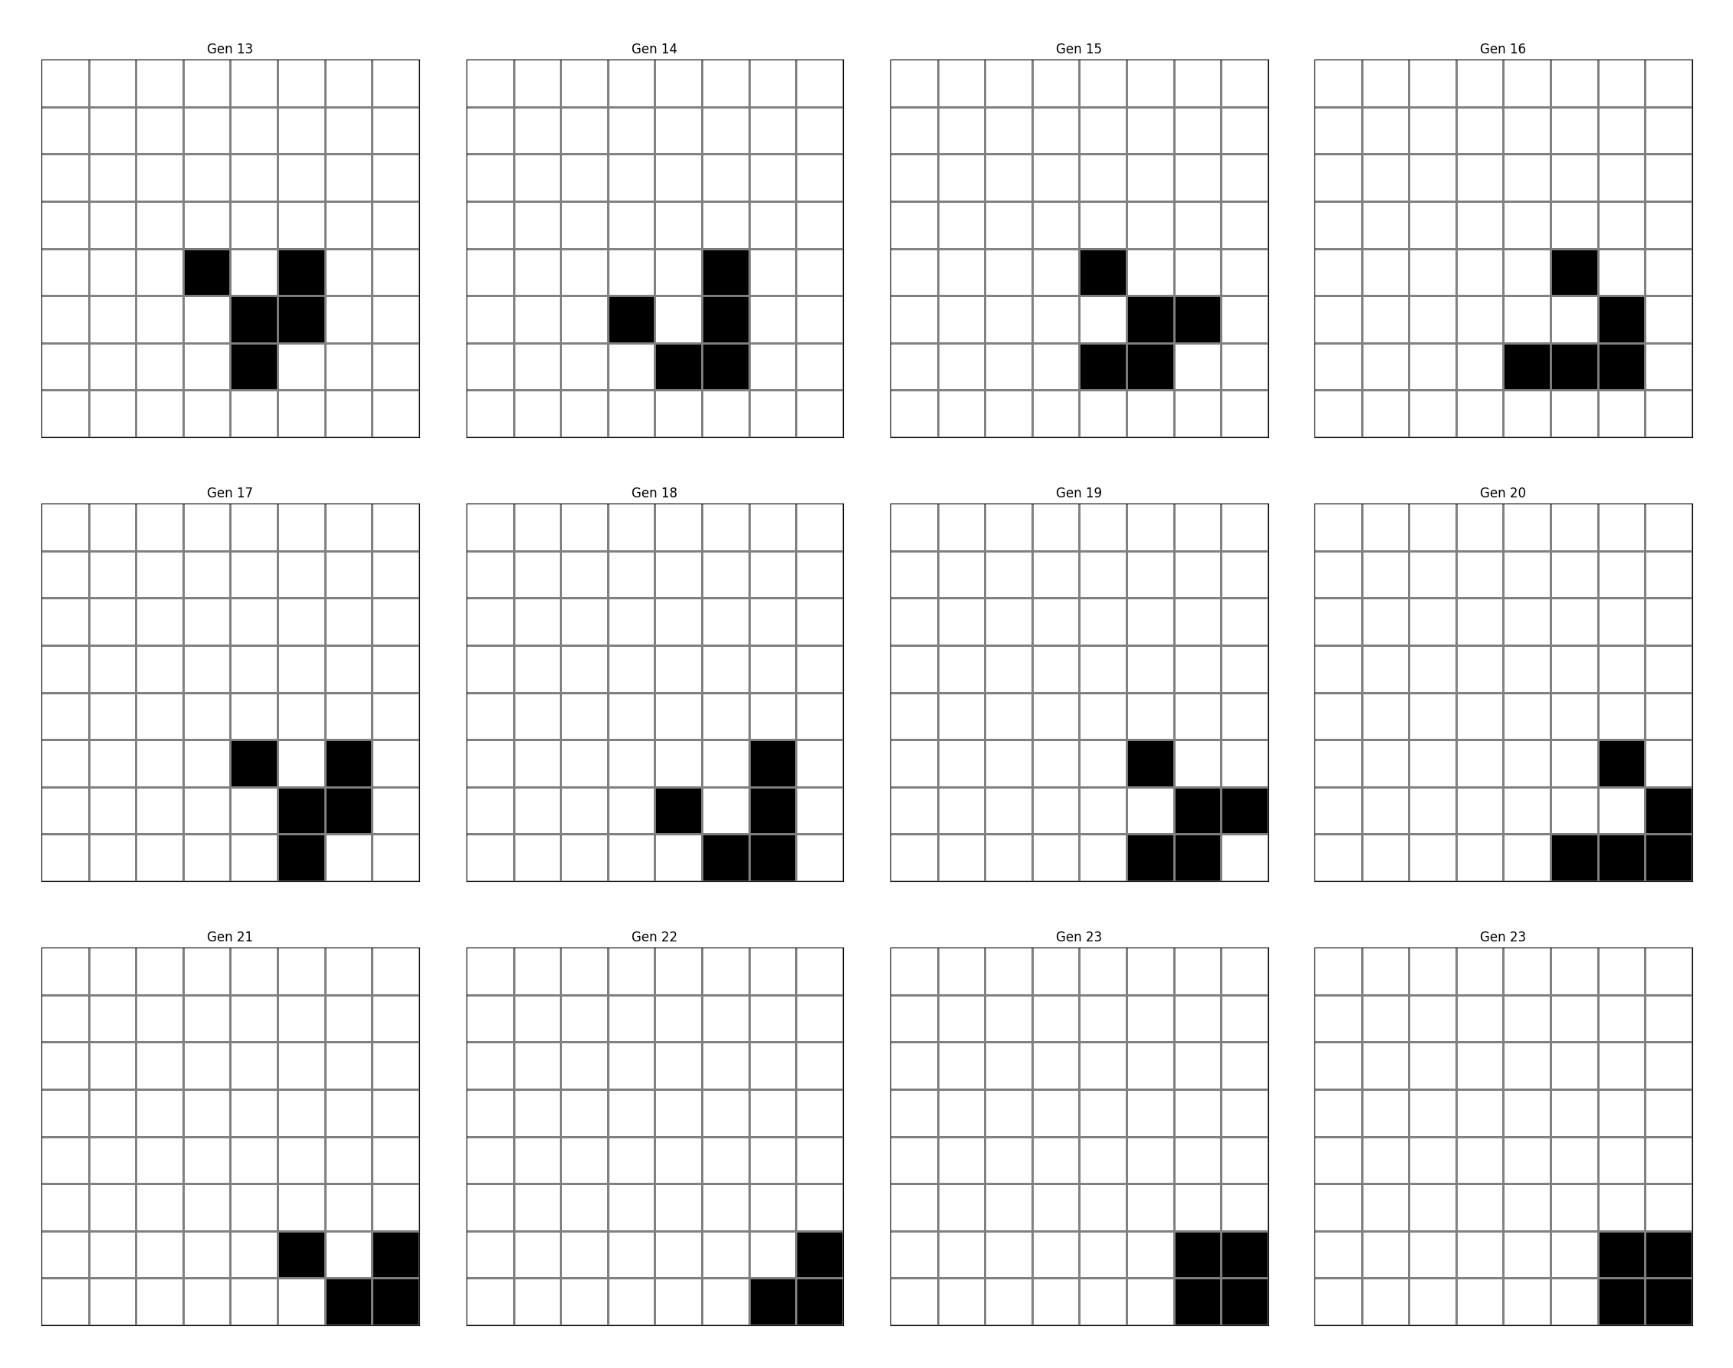
\includegraphics[width=0.87\textwidth]{../assets/space_ships/glider/glider_12_24.jpg}
  \caption{Patrón glider, generaciones 12-24: continúa su desplazamiento diagonal.}
  \label{fig:glider_12_24}
\end{figure}

\begin{figure}[H]
  \centering
  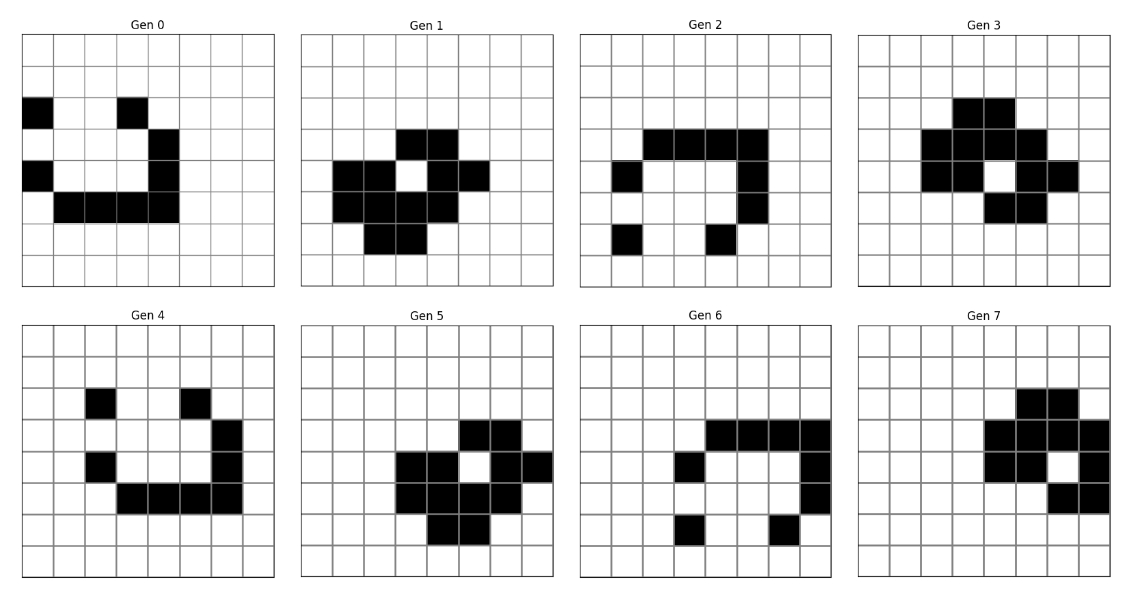
\includegraphics[width=1\textwidth]{../assets/space_ships/LWSS/LWSS.jpg}
  \caption{Patrón LWSS (Nave Ligera de Espacio Medio): una nave espacial que se desplaza horizontalmente mientras oscila en una secuencia de cuatro configuraciones.}
  \label{fig:LWS}
\end{figure}

\begin{figure}[H]
  \centering
  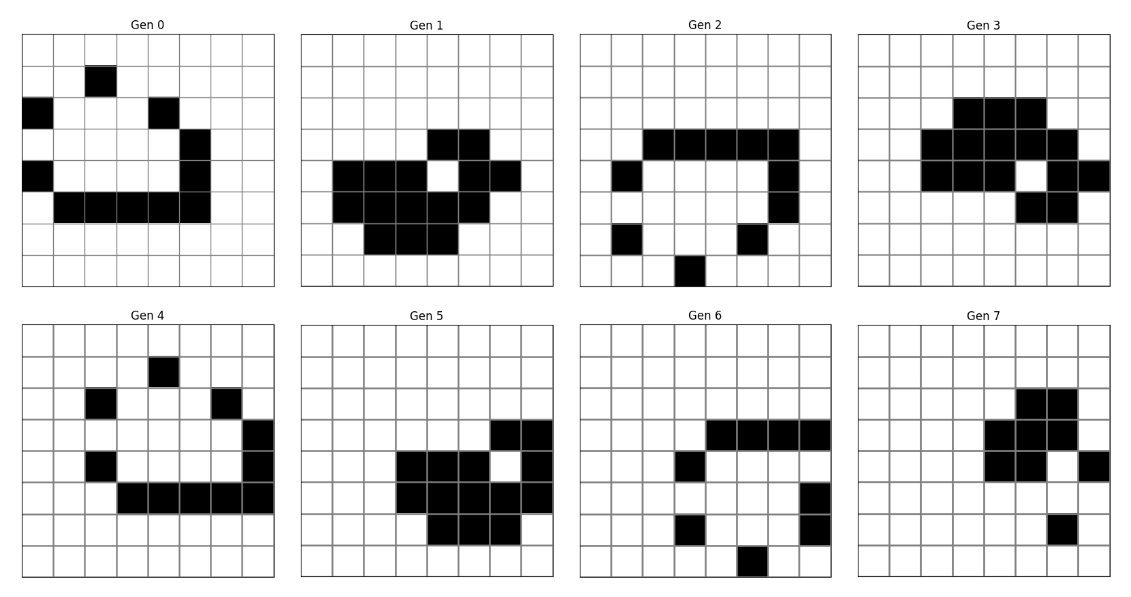
\includegraphics[width=1\textwidth]{../assets/space_ships/MWSS/MWSS.png}
  \caption{Patrón MWSS (Nave de Peso Medio del Espacio): se desplaza horizontalmente por el tablero, el tamaño intermedio entre las naves espaciales LWSS y HWSS.}
  \label{fig:MWSS}
\end{figure}

\begin{figure}[H]
  \centering
  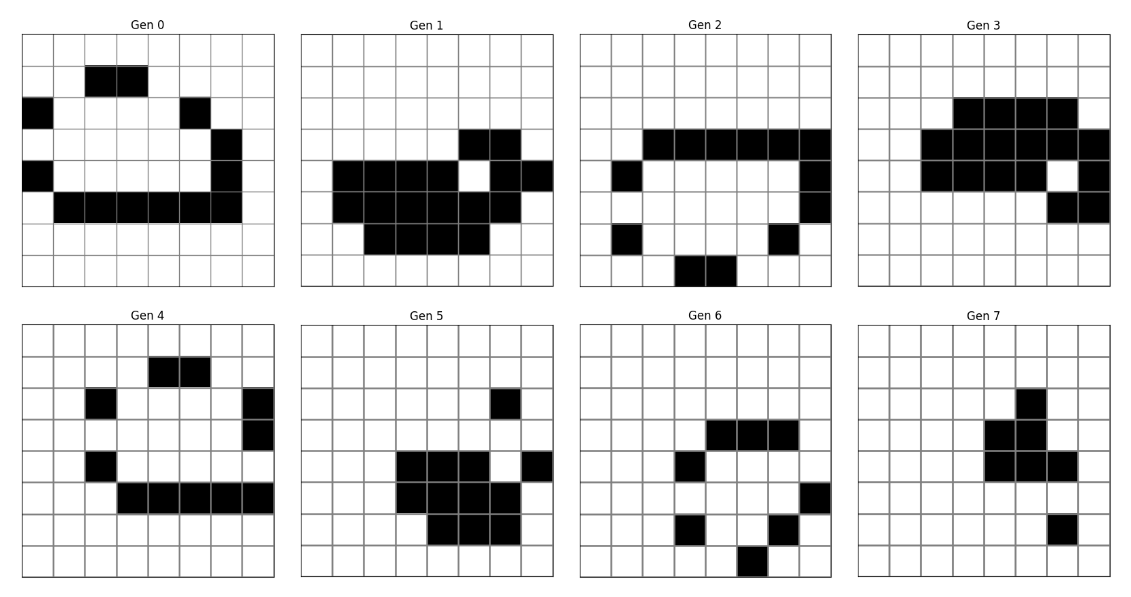
\includegraphics[width=1\textwidth]{../assets/space_ships/HWSS/HWSS.png}
  \caption{Patrón HWSS (Nave Pesada del Espacio): es la más grande de las tres naves espaciales básicas, se desplaza horizontalmente por el tablero hacia la derecha infinitamente.}
  \label{fig:HWS}
\end{figure}


\subsection{Methuselahs}
Los Methuselahs son patrones que evolucionan durante un número grande de generaciones antes de estabilizarse en un patrón estático, un oscilador o una nave espacial. El ejemplo más conocido es el "acorn", que evoluciona durante 5206 generaciones antes de estabilizarse en 633 células vivas, incluyendo 11 osciladores, 2 naves espaciales y 1 patrón estático.

% Aquí puedes insertar una figura de una nave ligera u otra nave espacial.

\subsection{Patrones Propios}
Sección dedicada a patrones que encontramos por accidente/pruebas.

\subsection{Patrones complejos}
Además de estos patrones simples, también existen patrones más complejos en el Juego de la Vida. Algunos de estos pueden "disparar" naves espaciales, otros pueden "construir" patrones adicionales, y otros pueden incluso comportarse como máquinas de Turing universales, lo que significa que pueden computar cualquier función computable.

% Aquí puedes insertar figuras de patrones complejos y discutir sus propiedades.

Estos patrones ilustran la increíble diversidad de comportamientos que pueden surgir del Juego de la Vida. En las siguientes secciones, veremos cómo estos patrones pueden ser generados e investigados usando PowerDEVS.



\section{Conclusiones}
\end{document}
